% !TeX root = ams_thesis.tex
\chapter{Implementation of Swarm Actions} \label{chapter:Implementation_of_Swarm_Actions}

The user interface may be able to drive the re-imagining of the robots as a unified swarm, and so alter the user's interaction with the swarm, by depicting the group in different ways \citep{manning2015heuristic}.
The base case is to simply display all the units as individuals, but this may not be useful for the operator \citep{coppin2012controlling}. 
Other approaches include an amorphous shape covering the area occupied by the swarm, an amorphous shape with density shading and motion arrows, the fields of influence for leaders in the swarm, and the web generated by the flow of information within the swarm. 
Considered as a whole, the swarm has properties, such as center of gravity or flock thickness, that do not exist in individual robots. 
Views of these properties may assist the user, for example in determining what areas have insufficient robot density for a thorough search operation. 

The information available to the user through the UI also implies the availability of certain information within the system. 
The distinction between UI representations of the swarm that display each robot as an individual robot versus those that display a cloud or amorphous shape in the area occupied by robots is the most obvious example. 
A system that displays the location of each robot must actually have localization information about each robot.
The presence of this information in turn implies that the localization information can be used to plan the actions of each robot, which in turn affects the structure of the programs generated for each robot. 

For example, if the task assigned to the swarm is to surround a fixed point, and localization information is available, then each robot can be given a program that instructs it to move towards a known location, based on its current known location.
Even if the robots cannot determine their location, but the UI and program generator have it, the robots closest to the point can be assigned programs that cause them to act as beacons, while all the other robots are assigned programs to wander until they see a beacon and then move towards it. 
If, instead, neither the robots nor the program generator have information on the location of the robots, then all of the robots can be assigned programs that instruct them to wander until they detect the target point, and then act as beacons, at which point the overall behavior of the system returns to the previous example.

In the most extreme case, neither the robots nor the user interface have any information about the location of the robots. 
As a consequence, the system could not display the individual robots situated in relation to each other on some form of map. 
This extreme is outside the scope of this work, as it is more suited to an interface that permits the provisioning of the robots with a description of the target point. 
A method for providing such a description through multitouch gestures is likely to be more tedious than other approaches, e.g. summarizing desired sensor precepts or including an image of the target area for the robots to recognize. 
However, if the user task is expressible in terms of the overhead view of the area, the user interface could simply allow the user to issue commands that are situated in that view, such as rallying at a certain point or moving an object that is visible in overhead view. 
Without information about the robot positions, the user would not be able to watch the motion of the robots to see that the commands were being followed. 

All of the valid expressions possible in the command language should be converted into programs for the robots, or the user must be usefully informed as to why it was not possible. 
The synthesized program should result in convergence of the swarm's overall behavior to the desired result. 
Clearly, in a developing situation in the real world, success may become impossible, and so there is not a practical way to guarantee that a particular valid command sequence will result in a particular desired state of the world. 
However, certain minimum bounds on the problem may be able to be used to determine if a desired task is certain to fail. 

\section{Localization}\label{sec:localization}

The initial vision for this work was to have minimal sensing and no localization. 
Minimal sensing results in a lower cost per robot, as it reduces the amount spent on sensors. 
Not relying on localization, especially localization via approaches such as GPS, which are easily blocked or interfered with, allows the resulting algorithms to be useful in situations where global localization is not available. 

However, a user interface that can display the swarm from an overhead view assumes that there is some form of localization, at least in terms of relative distances and bearings between the robots.
Without that information, the display of a group of robots in a way that matches their actual locations in the world is impossible, and displaying them incorrectly is likely to mislead the user. 
Even the unknown number of robots case assumes that the outer bounds of the swarm are at least approximately known. 

Fortunately for this work, there are a number of approaches to creating a local coordinate frame using robots with relatively simple sensors. 
A local coordinate system can be created by communicating agents with a limited, known sensing range but no other concept of distance \citep{bachrach2004experimental}.
One agent acts as a seed, and sends messages to its neighbours.
The neighbours propagate those messages, incrementing a hop counter in the message, and ignore messages with a higher hop count to stop the message from propagating backwards. 
As a result, each agent knows that its distance from the seed is at most the communication radius times the minimum hop count it has received. 
By using multiple seeds, each non-seed can calculate it's position based on trilateration to the seeds. 
Extending this method to use received signal strength as a proxy for distance, rather than the constant known sensing range, improves the accuracy of the approach.  
The Kilobot swarm uses a range-only sensor along with communication to create a local coordinate system \citep{Rubenstein795}.
A set of four stationary seed robots act as the origin of the coordinate system. As robots surround the four known robots, the new robot localizes from them and then begins broadcasting it's own position. 
Each new robot that joins the group uses trilateration to localize itself based on the robots that it can communicate with.

In addition to range-only approaches, bearing-only approaches to robot localization have been created, including an approach that uses the bearings to landmarks to create a vector field to drive the robot to a goal \citep{loizou2007biologically}. 
This approach is even able to guide an individual robot in the presence of moving landmarks. 
It does not, however, produce a coordinate frame that is shared among the robots, unless they somehow agree on the landmarks to use. 
A scale-free coordinate system can also be created using only bearing sensors and inter-robot communication, to arrive at a coordinate system that is shared among the robots \citep{cornejo2013scale}.
The addition of scale to such a system requires something beyond only bearing measurements. 
One way to do this is to use structure from motion (SfM) to estimate inter-agent distances, and use the measured distances to determine the scale for the network of robots \citep{spica2016active}. 
Alternatively, a pair of beacons of known location could provide the scale information required to convert scale-free coordinates into a metric coordinate system. 

Finally, systems that combine range and bearing information are common in swarm robotics \citep{arvin2009development, farrow2014miniature, caprari1998autonomous, mondada2009puck}. 
Systems with range and bearing can use trigonometry to calculate relative positions of other robots, and so can bootstrap a coordinate frame by using a method such as spreading inhibition to elect an origin robot, which then informs its neighbours of their positions in it's coordinate frame. The neighbours can then correct their position estimates based on communication with each other, as in range-based localization schemes, and inform their neighbours of their positions, propagating the coordinate system outward from the origin. 

As there already exist a large number of ways for robots to arrive at a local coordinate system without GPS or sophisticated sensors, the creation of a coordinate frame was determined to be outside of the scope of this work. 
Once the robots have developed a coordinate frame, the space the robots are in can be decomposed into a set of cells, and the program for the robots can be expressed in GCPR as checks on which cell the robot is located in and what the desired behaviour for the robot in that cell is. 
The desired behaviour for each cell is based on the user input on the interface device. Since the locations of the robots in the local coordinate system are known, and the location of the visualization of the robots on the user interface device is based on their positions in the local coordinate system, the user's input can be mapped into the local coordinate system to guide the robots. 
The combination of the spatial decomposition and the user input results in, essentially, a discrete vector field. 
By having the vectors in the field point towards a user supplied path, or along the path, the robots can follow the path using only their location in the local coordinate frame to guide them. 

Following the user-supplied path is important because it provides feedback to the user that the system is attempting to do what the user intended. 
In the simplest case, moving a robot to a target location, it could be argued that the thing that matters is that the robot arrive at the target location, rather than that it follow a specific path to get there. 
If a robot is in a bounded enclosure, and has a sensor that can detect when its goal is reached, the robot can reach the goal, or arbitrary close to it, by a random walk. 
If the robot can sense distance to the goal, it can find the direction of the goal by making a series of purposeful moves and samplings of the distance, and then go to the goal.
It could even approach the goal by performing a biased random walk. 
None of these approaches, however, would look to the user like the robot was following the path that the user provided, and so they are likely to confuse the user, leading to further control inputs as the user attempts to correct the robot. 
Additionally, the user's choice of path may be informed by knowledge that the user has, and that the robot may not be able to detect in the environment, such as areas that are inaccessible or dangerous to the robot. 
As such, the user's path selection can be viewed as an attempt to convey information about the desirability or utility of a given path to the robot, and so following the path given by the user is preferable to not following it. 

The space is decomposed into squares of uniform size. The size can be varied, but smaller squares result in a longer program for the robots and longer runtime for the decomposition algorithm. 
To determine the desired vector for a the cells of the spatial spatial decomposition, a multipass algorithm is used. 
The first pass assigns the vectors for those squares containing a point of the user specified path, or on the line between two points of the user path. 
Squares containing a point are assigned a vector pointing to the next point on the path. 
Squares between two points are assigned a vector pointing from the square center to the point closer to the end of the path. 
After this step, all points on the path have a vector pointing along the path. 
The second pass assigns to all squares neighbouring the end point of the path a vector pointed towards the end point of the path. 
As a result, the end point of the path becomes an attractor that robots attempt to reach. 
The third pass assigns to all squares that are adjacent to assigned squares a vector which is the average of all of the values of the assigned neighbors. 
This pass broadens the path so that it is greater than a single square wide, and ensures that the vector field around the path is smooth. 
The final pass is repeated until no square is assigned during a repetition. 
On each repetition, any square that is not assigned, but has assigned neighbors, is assigned the average of its neighbors and a vector from the center of the square to the closest point that is on the path. 
As a result, squares off the path drive the robot towards the path via the shortest route. 
When this pass is complete, every square of the decomposition of the space has been assigned a vector pointing in the direction that a robot in that square should move. 

The resulting decomposition can then be converted into a GCPR program by having each guard be a check on the position of the robot, and assignment of the robot's desired heading based on the grid square it is in.
A GCPR clause tells robots that are off their desired heading to rotate to that heading, and robots which are on their desired heading to move forward. 

Dispersion can be implemented in terms of vector fields as well. 
In the case of path following, every robot that was intended to follow the path would be issued the same decomposition of the space, but would follow different routes, as they start from different locations. 
To disperse the robots, each robot receives a different path, starting from their current location and moving to their new dispersed location. 
As described above, the robots can avoid each other while attempting to reach their new positions, and return to following their assigned paths once they are clear of each other. 
In implementation, the new locations were chosen by uniform random selection of points over the area the robots were in, but other approaches, such as positioning the robots so that each robot could communicate with at most two other robots, or on a regular grid in the local coordinate frame, would be amenable to the same implementation. 

These algorithms for path following and dispersion were implemented in ROS and tested in the ARGoS multi-robot simulator \citep{pinciroli2012argos}.

\section{Composition with Obstacle Avoidance} \label{section:Composition_with_Obstacle_Avoidance}

Reactive obstacle avoidance was initially added to the vector field program by only following the desired heading if the robot detects that it is not near any obstacles, and reacting to avoid the obstacles rather than follow the vector field if an obstacle is detected. 
This approach does have the weakness that the user can, for example, draw a path which passes through an obstacle. 
In a known environment, obstacles could be surrounded by repelling vectors, but in an unknown environment, this sort of command will cause the robots to approach the obstacle under vector field control, turn away from the obstacle until it is no longer visible, return to vector field control, and return to the obstacle. 
Even in a known environment, the local minima caused by ``U'' or ``C'' shaped obstacles present a problem for vector field based navigation. 

There exist a family of algorithims, called ``bug algorithms'', which provide complete path planning in a priori unknown environments with minimal sensing, under reasonable bounds, such as that the number of obstacles is finite and the goal is reachable. The bug family is large, and some of its members require sensing which may not hold in all conditions, such as location information or infinite-range distance sensing, but many do not. I-Bug, in particular, requires only the ability to detect a gradient which towards the goal and the ability to circumnavigate obstacles by e.g. wall following \citep{taylor2009bug}.

Generally, bug algorithms have two cases, the rules for motion in unobstructed space, and the rules for moving around obstacles. 
Rules for motion around obstacles frequently combine wall following around the perimeter of the obstacle with a leave condition that causes the robot to stop wall following and return to moving in open space. 
In the initial bug algorithm paper, the leave condition for Bug1 is to depart the obstacle from the point closest to the target, which requires circumnavigating the obstacle once to find that point \citep{lumelsky1987path}.

However, simply applying a bug algorithm to the movement of each robot in the swarm may result in undesirable behavior in a number of ways. 
First, many bug algorithms rely on wall following to pass around obstacles. 
If the other obstacle is another robot, operating under the same algorithm, the robots may begin to circumnavigate each other. 
If the leave condition for the circumnavigation is never met, this behavior would persist indefinitely. 
Under the leave rule discussed for Bug1, if one of the robots is moving slightly faster than the other, the resulting path of the two robots would be a spiral moving in some direction in space. 
Since Bug1 uses return to the same location to detect circumnavigation, and the spiral would never return to the same location, the leave condition would never be satisfied.

Further, it is important to include the path specified by the user in the path planning for members of the swarm. 
By following the path laid out for it, the behavior of the swarm is made legible by the human user. 
Compliance with the requested path indicates to the user that the swarm is under their control, and allows them to assess the progress of the system towards the goal. 
If, instead, the system uses some other form of path planning, it will initially appear to not be doing what the user requested, even if the end state does eventually become what the user intended. 
What factors contribute to this legibility and how best to balance them with other operational constraints of the system is beyond the scope of this paper, but has been examined in the context of manipulation, navigation around people, and combined in mobile manipulation around people \citep{dragan2015effects, kruse2013human, beetz2010generality}.
The work on legible manipulation also distinguishes between predictable motion, which makes sense to observers based on a known goal, and legible motion, which allows observers to infer an unknown goal. 
Extension of legibility and the emotive content of motion to swarm robots has also been recently investigated, but not in relation to human control of the swarm \citep{Dietz:2017:HPS:3027063.3053220}.

The user input may also contain information that is not available to the swarm, but is available to the user. 
This information may be necessary for the successful completion of the task, and so is not to be discarded lightly. 
For example, the optimal path in terms of minimal travel distance may be blocked by some transient condition, especially in the case of disaster response, such as fire or flood, and so the user may direct the robots to take a longer route to the goal. 
Discarding this information in favor of the shorter path could result in unit loss and mission failure. 

Unfortunately, composition with a vector field indicating the user-specified path to the goal with a bug algorithm for obstacle avoidance can break the guarantees of completeness that make bug algorithms appealing. 
For example, assume that the goal is a point with a vector field pointing towards that point from all locations in the operational area. 
A tempting bug algorithm for passing around obstacles is to circumnavigate the obstacle until the vector field points away from it, then leave and return to vector field control. 
For a simple polygonal obstacle between the robot and the goal, this results in reaching the obstacle, navigating some distance around it, and then departing it again on the side closer to the goal. 
However, if the the goal is surrounded by a right-handed spiral-shaped obstacle such that any straight line from the goal intersects the obstacle, the goal becomes unreachable. 
When a robot hits the spiral, it will wall follow in some direction.
If it uses a right-handed wall follow, it will reach the outer lip of the spiral and depart the obstacle following the vector field. It will then hit the obstacle again, since the vector field across the mouth of the spiral points towards the goal in its center, and begin wall following again. 
A left handed wall follow would reach the goal, but could be defeated by a left-handed spiral. 
Changing to randomly-selected lh- or rh-wall following changes the shape of the obstacles that can trap the robot, but does not remove the possibility, so long as the leave condition is simply that the vector field point away from the obstacle. 

\begin{figure}
	\centering
	\begin{subfigure}{0.45\textwidth}
		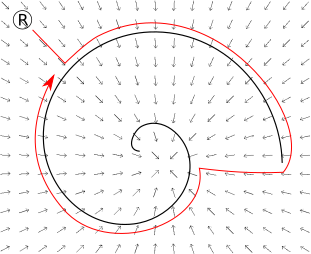
\includegraphics[width=\linewidth]{../spiral_trap.png}
	\end{subfigure}
	\begin{subfigure}{0.45\textwidth}
		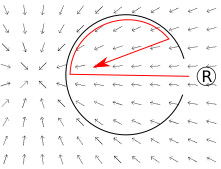
\includegraphics[width=\linewidth]{../wall_follow_trap.png}
	\end{subfigure}
	\caption{Simple obstacles that result in looping behavior for a bug algorithm that combines wall following with leaving the obstacle when the vector field points away from the obstacle.}
	\label{traps_for_wall_follow}
\end{figure}

In none of these cases is the goal unreachable, in that it is a member of the same set of points as the open space of the environment, but attempts at obstacle avoidance preclude the robot reaching it. 

\section{Code Generation Refinement}

Rather than rejecting bug algorithms because they cannot be usefully combined with a global vector field, the vector field representation of the space was rejected. 
Vector fields have other problems, beyond unsatisfactory composition with complete motion control planners such as the bug algorithm family. 
A vector field cannot represent a path that crosses itself, such as a patrol route that is a loop.
In the continuous case, a vector field is represented by a function that maps all points in the space to a vector representing the desired robot heading at that point. 
However, because a function produces exactly one value, each point can only have one heading, while the intersection point of a path has two headings, at different points in time. 
For a vector field broken up into discrete grid cells, the same problem applies, but to regions rather than points. 

One potential solution to this problem with vector fields is to have multiple vector fields, or multiple values at each point, and allow the robot to maintain a program counter, which it uses to determine which field or which value to use at a given point. 
The counter is incremented on departure from a vector field grid cell, and then on return to that cell, the new value of the program counter is used in a guard, which results in the robot using the second value of the heading. 

For example, the GCPR statements:\\
(self.is\_in((1.745, 1.921), (1.245, 1.421)) and pc\_is(1), self.set\_desired\_heading(2.332), 0.9)\\
(self.is\_in((1.745, 1.921), (1.245, 1.421)) and pc\_is(2), self.set\_desired\_heading(1.031), 0.9)\\
will result in the robot using the heading 2.332 when it passes through the grid region if the program counter is 1, and 1.031 when it passes through the grid region with the program counter set to 2 (while, unfortunately, not defining a desired heading if the program counter is set to some other value).

Using a program counter to select possible headings for a discrete vector field grid cell has the drawback that the program counter must be incremented on leaving the cell, as incrementing it while remaining in the cell will cause a change of heading.
As a result, the generated program must have guards on all cells surrounding the cell, which increment the program counter when triggered. 

Further adding to this complexity is the problem of sensor noise. 
If sensor noise causes the robot to erroneously detect that it has entered the neighboring cell, then the program counter could be incremented without the robot actually leaving its current cell. 
On the next update of the noisy position sensor, the robot could then ``return'' to the current cell, and change direction due to the incorrectly implemented program counter. 

As a consequence of the complexity attendant on repairing the inability of the vector field to represent paths containing loops, the underlying representation of the conversion of user paths into robot programs was changed to avoid the use of vector fields. 

\subsection{Approaching a Point}

The basic action of the robot is to move from one location to another. 
Under the assumption that there exists some form of localization, which must hold in order to support the type of user interface described in this work, the simplest approach to navigation to a point is for the robot to rotate to face that point and then move forwards towards it. Once the point is reached, the robot should stop. 

Reaching of a point is more complex for swarm robots than it is for single robots. 
Some work assumes that robots in the abstract are points, and as they occupy no area, any number of them may congregate at a mathematical point. 
In the real world, while a point may be described precisely, it is usually sufficient to arrive within some small distance $\epsilon$ of it to say that the robot has reached the point. 
However, robots also take up space in the real world, and so as more and more members of the swarm arrive at the point, the later arrivals may be precluded from actually approaching to within $\epsilon$ of the point.
In this case, it is desirable to have a definition of arrival that expands to allow robots to approach the point as closely as they can and stop when that condition is met. 

For example, when a robot arrives at the point, it might stop, but broadcast a message to local robots that it is at the point. 
Robots arriving after the first would then navigate around it, keeping track of the minimum distance to the goal. 
After finishing a circumnavigation, the robot would then return to the closest point to the goal. 
As more robots arrive, the local minimum in the approach to the target point may become occupied by another robot, and so if that point is occupied, the robot would then have to perform another circumnavigation to find a new closest point. 
Because every iteration of this loop either occupies the closest point with a robot, or detects that the closest point has become occupied by another robot, and triggers another iteration, it will eventually position every robot as close as possible to the goal. 

\section{Completeness of Navigation}

Moving to a point is implemented as a bug algorithm. As described earlier, bug algorithms are complete, in that they navigate the robot to a point, or determine that the point cannot be reached. A review of eleven bug algorithms can be found in \citep{ng2007performance}. 
Bug algorithms also generally rely on only local sensing and minimal data storage, and so are appealing for use in swarm control. 
In this section, the basic bug algorithms are extended to determine if it is possible to provide local-sensing-based complete algorithms for the tasks from the user test. 

Unfortunately, most of the bug algorithms have the requirement that the obstacles in the environment are not moving.
Indeed, the presence of moving obstacles results in navigation becoming undecidable without knowledge of the future movement of the obstacles, as an obstacle can move to occupy the robot's goal. 
Unless it is known whether the obstacle will move off the goal in the future, it cannot be determined whether the goal is unreachable, or just not currently reachable. 

The Tangent-bug algorithm has been extended to handle moving obstacles, given a number of constraints \citep{kamon1998tangentbug, tomita2009sensor}.
The main constraint that affects the use of this algorithm is that the obstacles are constrained to be moving at a velocity that is slower than that of the robot.
This constraint is required because if the robot is circumnavigating the obstacle, and the obstacle is moving faster than the robot, then in the time that the robot requires to circumnavigate the perimeter of the obstacle, the obstacle will have moved a distance greater than its own perimeter is long, and the circumnavigating robot will have moved with it.
As a consequence, the circumnavigating robot might not return to its own previous path and cross it, which is the condition that Tomita and Yamamoto use to determine that the robot should leave the obstacle. 

At first, this would appear to be a problem for swarm robots, because if the robots are the same, they will be moving at the same speed. 
If one moves in a straight line, and the other attempts to circumnavigate it, the circumnavigating robot will never cross its own path for the reason described above, and so never leave. 
However, if the robots are using the same bug algorithm, this trap will not be sprung, because each robot will attempt to circumnavigate the other. 
If they attempt to circumnavigate each other in opposite directions, they will spiral around each other, leading to at least one of the robots crossing its own previous path, and triggering the leave condition of the algorithm. 
If they attempt to circumnavigate each other in the same direction, they will come to a position side-by-side, as neither can outpace the other, but neither will pull away from the other because they are attempting to follow each other's perimeters. 
In this case, they are pointed towards the goal, because in the absence of an obstacle, Tomita and Yamamoto's modified Tangent-bug orients the robot towards the goal, and so before they encountered each other, the robots were oriented towards the goal.
The robots will then approach the goal, and one will arrive, while the other circumnavigates the first until it detects that it cannot arrive at the goal. 

Tomita and Yamamoto do not deal with the decidability of their modification of Tangent-bug because they constrain the goal point to be not within an obstacle, and so reachable by the robot. The original Tangent-bug will navigate the robot to the goal if it is reachable, or circumnavigate the obstacle, returning to its starting point, whereupon it detects that the point is unreachable \citep{kamon1998tangentbug}. Since Tomita and Yamamoto constrain the goal to not be within an obstacle, the original Tangent-bug will reach it. 

In the case of moving obstacles, if the goal is covered by an obstacle, the obstacle is either moving or not moving. If the obstacle is moving, the modified Tangent-bug will not return to its original hit point, which is either left behind or covered by the obstacle, but will eventually cross itself, and leave the object towards the goal.
If the obstacle is still covering the goal, this process will repeat until the object is not covering the goal anymore, and the robot will reach the goal. 

In the case of swarm robots, as described above, some mechanism may be needed to determine that the goal is occupied, possibly by other swarm members, and to stop at a location near the goal. 
The stopping condition of the original Tangent-bug in the case where the goal is unreachable extends naturally to swarm robots. 

If a robot is the first to arrive at the goal, the goal is not occupied, so the robot occupies it and stops. 
If a robot is not first to arrive at the goal, the goal is occupied by a robot, which is stopped. 
The new arrival treats the stopped robot as an obstacle, circumnavigates it, returns to the original hit point and so detects that the goal is unreachable, and stops. 
If multiple new arrivals get to the stopped robot(s) at the same time, the conditions above hold, and so they eventually either cross their own paths while trying to circumnavigate another robot that is also circumnavigating an obstacle, and so leave and return (and so become later arrivals), or complete a circumnavigation and return to their own starting point and stop (becoming part of the obstacle).

If a maximally dense cluster of robots is desired, the unreachability check of Tangent-bug can be extended. 
Once the goal is determined to be unreachable, the robot performs another circumnavigation of the blocking obstacle to find the closest point to the goal, and returns to that point. 
That point has either been occupied by another robot, in which case the robot repeats this step, or occupies that point if it is free. 
Because every iteration of this step fills the point closest to the goal with a robot, the resulting cluster of robots is packed as close to the goal as possible. 

 \begin{figure}
 	\centering
 	\digraph[scale=0.6]{TangentBugMod}{
 		
 		start -> obstacleToGoal;
 		obstacleToGoal -> aimToGoal [label="No"];
 		aimToGoal -> atGoal;
 		atGoal -> stop [label="Yes"]; 
 		atGoal -> obstacleToGoal [label="No"];
 		obstacleToGoal -> recordHit  [label="Yes"];
 		recordHit -> followEdge;
 		followEdge -> closerPoint;
 		closerPoint -> leaveObstacle [label="Yes"];
 		leaveObstacle -> obstacleToGoal;
 		closerPoint -> pathCross [label="No"];
 		pathCross -> returnToHit [label="No", color="blue"];
 		returnToHit -> followEdge [label="No", color="blue"];
 		returnToHit -> unreachable [label="Yes", color="blue"];
 		unreachable -> lastPoint [color="blue"];
 		lastPoint -> updateGoal  [label="No", color="blue"];
 		lastPoint -> stop  [label="Yes", color="blue"];
 		updateGoal -> obstacleToGoal [color="blue"];
 		pathCross -> obstacleToGoal3 [label="Yes"];		
		obstacleToGoal3 -> followEdge2 [label="Yes"];		
		obstacleToGoal3 -> aimToGoal[label="No"];		
		followEdge2 -> obstacleToGoal3;
		
 		obstacleToGoal [label="Obstacle in direction of goal?"];
 		aimToGoal [label="Orient towards and move to goal"];
 		atGoal [label="At goal?"];
 		leaveObstacle[label="Leave obstacle"];
 		recordHit [label="Record hit point"];
 		unreachable [label="Goal is unreachable", color="blue"];
 		updateGoal [label="Next point is new goal", color="blue"];
 		lastPoint [label="Is this the last point?", color="blue"];
 		followEdge [label="Follow obstacle edge"];
 		returnToHit [label="Returned to hit point?", color="blue"];
 		closerPoint [label="Closer to goal than hit point?"];
 		pathCross [label="Crossed own path?"];
 		obstacleToGoal3 [label="Obstacle in direction of goal?"];
 		followEdge2 [label="Follow obstacle edge"];
 	}
 	\caption{The proposed modifications (in blue) to the Tomita and Yamamoto Tangent-bug algorithm for user path following in cases with multiple robots, some of which may be treated as moving obstacles. This flow chart does not include the option for maximally dense packing at the goal described in the text. }
 \end{figure}

\subsection{Path Following}

As discused previously, it is desirable to have the robots follow user-defined paths rather than simply determining what the end position of the robots is to be and heading directly to that point. 
The reasons for this are twofold:
\begin{enumerate}
	\item Following the user path makes it clear to the user that the robots are doing as the user directed. 
	\item The user path may be chosen as a consequence of information that the user has and that the robots do not, and so satisfies some property other than simply arriving at the goal, such as avoiding a dangerous area or providing a sensor sweep of an unexamined area. 
\end{enumerate}

A user path can be followed by a bug algorithm by breaking the user path into a series of points, and using a bug algorithm to navigate to each point in turn. 
Because the bug algorithm is complete, it can either reach the target point, or determine in finite time that the point is not reachable. 
Path following can be handled as an iterated application of the bug algorithm for motion to a point.
The path is represented as a sequence of points, ending with the goal point.
Rather than terminating when a point is either reached or determined to be unreachable, the algorithm changes the goal to be the next point of the user path. 
Motion to the goal point is complete, as it is simply tangent-bug navigation to a point and tangent-bug navigation has been demonstrated to be complete under reasonable constraints. 
Motion to the point prior to the goal point can either reach the prior point, or detect that it is unreachable. 
In either case, the algorithm then transitions to attempting to reach the goal point, which has been demonstrated to be complete.
Since motion to the point before the goal is guaranteed to transition to a complete approach to the goal, it does not alter the completeness of the algorithm. 
The same logic holds for each point prior to the attempt to reach the goal point, and so the entire path following algorithm is complete.  

However, the path followed by the robot may miss one or more of the user-defined points, and in fact may miss all of them, if, for example, the entire user path happens to be within a previously undiscovered obstacle.  
The upper bound on the length of the path that tangent bug will produce is given by 
\[P_{max} = ||S-G|| + \sum_{i}\mathsmaller{\prod_i} + \sum_{i}\mathsmaller{\prod_i} \times \#Minima_i \]
where $||S-G||$ is the straight line distance from the start to the goal, $\prod_i$ is the perimeter of the $i^{th}$ object, over all objects $i$ in the disk with radius $||S-G||$ centered at the goal, and $\#Minima_i$ is the count of local minima in distance to the goal on the perimeter of the $i^{th}$ object. 
In the case of iterated tangent bug, this bound is then summed over each goal point. 
While the perimeters of the objects are constrained to be finite in order for tangent bug to converge, they may be very large, and so send the robot far from the user path. 
Whether this deviation is acceptable or not depends on factors outside of the scope of \emph{a priori} algorithm development, such as the parameters of the mission that the user is sending the robots on, and so is not amenable to solution here. 

\subsection{Formation}

In the user interface tests, the formation task was to cause the robots to form a formation, but did not involve motion in formation. 
It was not specified whether the formation was to be a form of aggregation which constrains the robots to be within the perimeter of the desired formation, or if the robots were required to be on the perimeter of the formation, with no robots inside or outside of the formation area. 

In the case of robots with localization, the formation can be sent to the robots as a list of points, similar to how a path would be sent to the robots as a list of points, and the robots can select points that are either inside that formation or on its edge, as needed, and then follow paths to those points. 
However, such a naive algorithm could result in the loss of the completeness properties of the bug algorithm if failure to reach the target point is handled poorly. 
If the robot simply selects a new point each time its target point is not reachable, and no point in the formation is reachable, then the algorithm will loop forever. 

Instead, the path following behavior can be adapted to generate a path that will position the robot on the perimeter of the formation, or determine that such a positioning is impossible.
The formation algorithm consists of two phases, approach to the perimeter and positioning along it. 
Approaching the perimeter is done as in path following, with the perimeter points serving as the list of points on the path. 
As with path following, the robot will attempt to reach each point along the perimeter in turn, and if none of them are reachable, the algorithm will terminate, having determined that the entire perimeter of the formation is inaccessible. 
However, once the robot reaches any point on the perimeter, there are two options for the algorithm. 
The robot can stop, as it is now on the perimeter and so ``in formation''. 
Any subsequent robot following the path will then treat that point on the path as blocked by an obstacle, and proceed to attempt to reach the next point. 
As a result, each robot stops at the first unoccupied space on the path, or fails to find any unoccupied spaces and terminates upon failure to reach the last point in the path. 
Alternatively, the robot could stop when it reaches the last point, or, on failure, backtrack to the last point that it could reach.% \todo{is it valuable to attempt to explore the entire formation before picking a spot?} 
In either case, as with basic path following, the algorithm is complete. 

Interestingly, the Bug2 algorithm from the original work on bug algorithms is a better choice for the basic bug algorithm used this style of formation than the modified tangent bug algorithm \citep{lumelsky1987path}. 
While tangent bug does have a lower bound than Bug2 on the maximum path length, Bug2 uses a path called the m-line which is the line segment passing between the start point and the target point.
For a polygonal formation expressed as a list of points, the m-lines between each subsequent set of points form the perimeter of the formation. 
As a result, any point which is on an m-line and in free space, rather than within an obstacle, is a valid point for the robot to stop on and consider itself ``in formation''. 

The use of bug algorithms as outlined here does not address the problem of dispersion along the edge of a formation. 
A reasonable expectation of the behavior of a swarm commanded to form e.g. a square shaped formation is that the robots would be approximately evenly distributed along the perimeter of the square, at least where there were no obstacles to prevent it. 
Having the robots all located around one corner of the square or along one edge, while technically on the perimeter, would be less satisfactory. 
There are a number of possible approaches to spacing along the formation perimeter that might be adopted, depending on the robots' sensing abilities.
Since the basis of this work includes a central user interface which generates the robot programs and transmits them to the individual robots, one way to distribute the robots would be to base the decomposition of the formation perimeter into segments based on the number of robots available, and have each robot's final path point be a different point on the formation perimeter. 
If the programs used the second alternative for stopping at unoccupied points while following the perimeter, they would preferentially take their final path point, and fall back into each other's path final points if their own was unavailable.

If the robots can sense each other, they could disperse along the perimeter according to some higher-level rules for setting their own goals, but using bug algorithms to navigate. 
For example, if it is known that enough robots exist to cover the perimeter tightly enough that every robot can see a robot to its left and right, bounded by some limited sensing radius, robots could move on the perimeter to keep the distances between the robots to their left and right equal, treating points where obstacles intersect the perimeter as robots.
However, if the unobstructed perimeter of the formation is greater than the twice the robots' sensing radius times the number of robots, gaps in the perimeter will lead to oscillation as robots attempt to fill them. 
Lacking a global knowledge of the situation, the robots cannot determine that the perimeter is unfilled. 

\subsection{Patrol}

Patrol is distinct from the other tasks because it has an infinite loop in it by design. The robots patrol the area, and once they finish the patrol, they begin again. 
A complete algorithm is one which will either obtains the correct result, if possible, or indicates failure. 
In either case, a complete algorithm terminates, while a patrol does not. 
However, the navigation algorithm can simply be the same as the path algorithm, only looping over the list of goal points rather than passing through each of them once. 
While not complete because it does not terminate, each attempt to reach a point on the patrol path is complete, in the sense that it either reaches the point, or determines that it cannot be reached. 
The algorithm moves on to the next point in either case, rather than terminating. 

In a non-dynamic environment, obstacle-free environment, the algorithm will cause the robot to arrive at every point of the patrol path, since there are no obstacles to prevent it.
Adding obstacles raises the possibility that the robot may have to deviate from the patrol route to circumnavigate obstacles. 
As a result, while the robot will attempt to reach all of the points in the patrol loop, it may miss any or all of them due to obstacles. 
In this case there needs to be some sort of criterion for how bad the deviations from the patrol route can be and still be regarded as a satisfactory patrol.
Since this criterion is most likely something related to the overall goals of the user, such as detecting the approach of some other actor to the patrol area, the failure of the criterion is unlikely to be detected by the individual robots. 
Instead, the detection of failure to reach patrol points should be propagated back to the user in a way that allows the user to decide if the patrol path is still acceptable. 

Adding dynamism to the environment raises a concern with the modifications of tangent bug required to allow it to operate in a dynamic environment. 
In the modified tangent bug, a robot crossing its own path is caused by a dynamic obstacle, but in the case of a patrol, the robot constantly crosses its own path. 
In order to detect the path crossings, the modified tangent bug of Tomita and Yamamoto keeps track of its own past locations, and detects the intersection of its current location and next position with each line segment between each of its own past locations. 
However, this problem is not as dire as might be expected. 
Because the path following is considered an iterative application of the modified tangent bug, the buffer of previous path locations is cleared on beginning the next iteration, which is caused by either arriving at a goal or determining that the goal is unreachable. 
This also greatly reduces the storage requirements for the path, as not all points along the path are required to be stored, and allows the user path to have loops, which motivated the use of modified tangent-bug to begin with. 

\subsection{Dispersion}

Dispersion can be treated as movement to points, but the selection of points can be handled in a number of ways. 
If the robots can communicate and are localized, they can agree on a dispersion based on e.g. the space covered by the swarm and a desired density. 
As with formation, each robot could be assigned a target point to disperse to.
Unlike formation, the primary concern is that the robots be evenly spread throughout the area, rather than within or along a specific perimeter. 
However, in the presence of obstacles, attempts to approach the target points could be thwarted by inter-robot interference. 
For example, if many of the dispersion points are within an obstacle, and one is in the only, narrow corridor into that obstacle, the arrival at the robot assigned to the corridor dispersion point will block all the others from arriving at their dispersion points. 
Because of this problem, it is preferable to have each robot be able to determine whether the dispersion is at least locally complete, rather than rely on simple arrival at a point to regard itself as ``dispersed''.

Unfortunately, this change renders dispersion more complex than formation. 
While a single robot may have some way to detect that it is ``in formation'', such as being at a point within a polygon, it has no way to detect that it is dispersed, and indeed, it makes little sense to talk about a single robot being dispersed. 

Dispersion is, instead, a state of the swarm as a whole, rather than the state of a single robot. 
If the robots can sense each other, it becomes easier, because they can at least determine if they have neighbors, or possibly how far their neighbors are away, and so can examine local conditions of dispersion. If all robots can detect that in their local area, they are well-dispersed, and all robots act to be locally well-dispersed, then the swarm as a whole will tend towards being well dispersed. 
For the purposes of further discussion, the definition of ``dispersion'' is that for some integer threshold $\alpha$ and some finite sensing radius $r$, there are no more than $\alpha$ other robots within $r$. 
This definition has some limitations, such as regarding a single robot ``swarm'' as permanently dispersed. 
For the purposes of this argument, we will assume robots are points, but aside from some degenerate cases, the argument can be shown to generalize to robots with area. 
Point robots raise the problem that if $\alpha$ is allowed to equal the number of other robots in the swarm, then all of the robots in the swarm are permitted to be arbitrarily close to each other within $r$, and so the criterion will consider a state with all robots occupying the same point to be ``dispersed''. 
This is counter to the intuitive understanding of dispersal, and so $\alpha$ is constrained to be less than the number of robots in the swarm. 
%This runs into the paradox of the heap. 
%How much lower than the number of robots in the swarm must $\alpha$ be for the robots to be considered dispersed. 
%\todo{hexagonal close packing of circles of radius r, so 6 seems to be the upper bound, beyond which there is some other kind of problem}.

It may be that dispersion cannot be performed, for example due to limited space in the area to be dispersed into. 
In order to derive a complete local-sensing-only dispersion algorithm, the algorithm must be shown to move every robot to a location where the robot can detect using local sensing that it is dispersed, or determine that such a location does not exist.

For two robots and $\alpha = 0$, there must exist two points in the space such that the distance between those points is greater than $r$. 
Because the sensing range of the robots is $r$, a robot located at a point cannot tell if a point greater than $r$ distance away is unoccupied, and so the algorithm requires some form of non-local sensing, either communication with other robots or map building. 
In fact, in order to determine that there exists no such pair of points in the space, the robots must be aware of all the accessible points in the space, which amounts to global, rather than local knowledge.%\todo {is this correct?} 
For two robots, $\alpha$ may not be increased, as it would then violate the constraint that $\alpha$ be less than the number of other robots in the swarm. 

If the number of robots in the swarm is increased by one, the number of points in the space that are required to be greater than $r$ apart increases by one. 
If $\alpha$ is increased by one, allowing one robot to be within $r$ of another robot, then the problem reduces to the two robot case with $\alpha=0$ and the third robot able to be placed anywhere. 
However, as the two robot case requires global sensing to determine whether there exist two points that are greater than $r$ apart from each other, it is still not a complete local-sensing-only algorithm. 

For any number of robots $M$ and $\alpha < M$, split the swarm into a group of $\alpha$ robots and and the remaining $M - \alpha$ robots. 
Because $\alpha$ robots may be within $r$ of each other, put them all at the same arbitrarily selected point. 
The remaining $M - \alpha$ robots must be placed at points that are more than $r$ from that point, or else the group of size $\alpha$ will have more than $\alpha$ robots within $r$ of them.
As with the two-robot case, determining that there does not exist an accessible point greater than $r$ distance from any point in the space requires global information about the space. 
As a consequence, a complete local-sensing-only dispersion controller for point robots does not exist.
It either requires global information, in which case it is not local-only, or it cannot determine that a satisfactory target point does or does not exist, and so it is not complete.

Making the robots take up space, rather than being points, can result in the condition that $\alpha$ robots simply cannot fit within the disc of radius $r$ around one robot (for example, if the robot radius is $r$), and so even close-packing of the robots is considered ``dispersed".
Leaving aside this degeneracy, if $\alpha + 1$ robots can fit within $r$ of one robot, and $\alpha$ is constrained to be less than $M$, then the extra robot is required to be greater than $r$ from the surrounded robot, and the same argument holds with regard to determining if a point greater than $r$ distance from the surrounded robot exists or not for all possible placements of the surrounded robot.

Despite the fact that a complete, local-only dispersion controller cannot be found, there are controllers for dispersion of robots that are proven to converge, and to operate without localization \cite{correll2009ad}. 
This style of dispersion does require that the robots be able to detect and communicate with each other.
With non-communicating, non-localized robots that can detect range to other objects, e.g. via intensity of reflected light, dispersion over an area can be accomplished by having all robots move to keep all objects that they can detect within a fixed range.
Even simpler, robots could travel towards open space until they detect no surrounding objects and then stop, or stop if they detect no open space.  
Varying the detection range will the density of the swarm, both in terms of distance from each other and from obstacles. 

\subsection{Swarm Manipulation}

One interesting minimum case for transportation is the use of granular convection to transport an object that is larger than the robots to a goal, without inter-robot communication or sensing beyond a weak repulsion from the goal \citep{sugawara2014object}. 
However, this form of box-pushing has some limitations, such as the space being enclosed, and the shape of the transported object being such that it cannot become trapped against the sides of the enclosed space.

Another possible approach is the use of occlusion-based transportation \citep{chen2015occlusion}. 
The robots push on the object if the object is between them and the goal, and so occludes their view of it. 
By adding a moving goal, as in the case of path following via bug algorithms as discussed earlier, this transportation method can even cope with environments where the eventual goal is not visible from the starting point. 
The user-supplied path, expressed as a sequence of goals, provides information on the obstacle-free route through the space. 
Again, this form of transportation is prone to failure in the case of the object arriving an a position where one face of it is against a wall, and so no robot can get behind it to push it off the wall. 
It is also only proven to work for arbitrarily shaped convex objects. Certain pathological concave objects can actually result in a net force away from the goal. 

The use of simple sensors can be used to coordinate multiple robots to move a box to an illuminated goal \citep{kube1996use}. 
Kube and Hong used sensors to track a light on the box and distinguish the box from other, unlit boxes, which were treated as obstacles. 
If distinguishing obstacles is unnecessary, the robot could simply use two light sensors, and push forward if the lower one is occluded by the box and the higher one can see the goal. 
However, such a simple robot will push against obstacles that cannot move, and other robots. 

It would be good to determine if manipulation in this style, which is to say simple pushing rather than caging or pulling manipulation, admits a complete controller as path following and formation do, or if it is not possible to, in finite time, either move an object to a goal, or determine that it is not possible. 
For the purposes of this argument, it will be assumed that the object can be pushed in any direction, and that there are sufficient robots present to push it. 
In reality, it is possible that the object cannot be pushed at all, or that constraints on its dynamics render it impossible to push it to the desired location. 
For example, it is possible for a human to push a car with its gearbox in neutral forward or backwards, but not sideways. 

In unlimited free space, it is clearly possible to push an object to the goal.
The robot must be able to locate the object and goal in some way, but as discussed by Kube and Hong, the required sensor precepts may be fairly simple even for real robots. 

In bounded free space, there is the possibility that the object can be placed against the boundary of the space in such a way that no pushing force can remove it from the wall again. 
For example, an oblique triangle with one face against a straight wall is pushed towards the wall by forces normal to its exposed faces. 
Of course, under some conditions of friction and pushing forces, the triangle may rotate away from the wall, but as the length of the wall-facing side grows, the more normal the forces become to the wall itself, and so at some point the friction against the wall will exceed the pushing force of the robots on its sides. 

Using only local sensing, it is possible to detect this sort of stuck condition, and indicate that the attempt has failed. 
If the robot detects that it is pushing the object, but the robot is not moving, then the object is also not moving. 
If the robot then circumnavigates the object and is able to pass from the object to an obstacle and back, then one side of the object is against the wall. 
Note that this may require the robot to also circumnavigate the boundary of the space, if the object is against a wall, which may be large. 
It also assumes that the robot can detect its own motion. 

In an unbounded space with obstacles, the object may be able to be pushed to the goal if there is an unoccupied path that the object can pass through in order to arrive at the goal. 
While having a clear path is a necessary condition, it is not sufficient. 
For example, if a square object is being pushed down a corridor that is exactly wide enough to admit the square, and has a 90$^{\circ}$ bend in it, the square will fill the bend and become stuck, as no pushing force on either of its exposed faces will move it in either direction along the corridor. 
Nonetheless, the corridor is wide enough to admit the square, and so even if traversing the corridor is required to get to the goal, it does not violate the condition that there be an unoccupied free path that the object can pass through in order to reach the goal. 
Further, being able to detect such a path requires being able to check assertions about distances across sets of points throughout the space, and so global, rather than local, sensing or knowledge. 

By adding various levels of communication, more complex sensing, and global planning to the capabilities of the robots, autonomous box pushing can be performed under different conditions. 
A review of these techniques is beyond the scope of this section, but for recent results see \citep{tuci2018cooperative, rahimi2018comparison, alkilabi2017cooperative}. 
Occlusion-based transportation, on the other hand, is effective with minimal sensing, and as discussed above, similar bug-algorithm-based path following. 

Users frequently positioned robots near the object or used a dragging action of the box itself in the interface, so the path for the robots to follow is defined as the list of points that the user dragged over. 
However, the robot's goal is no longer to arrive at the destination.
Instead, the robot's goal is to arrive at the box and circumnavigate it while detecting the points where the line between the robot's location and the goal (the m-line in the Bug2 algorithm) passes through the box. 
If there are no points where the m-line does not pass through the object, then the object is sitting on the goal and the robot should stop. 
If there are points where the m-line does not pass through the object, then the robot should return to a point where the m-line does pass through the object, and push there. 
If there are no points where the m-line passes through the object, the object has a hole in it with both the goal and the robot in it, and the robot can sit still, as the object is already surrounding the goal.
This algorithm does not detect arrival at the point, but will instead cause the robots to push the object back and forth over the goal. 
If enough robots are present, the object will stagnate at the goal as the forces of the robots on all sides of it come into balance as indicated in by Chen et al. \cite{chen2015occlusion}.

Unfortunately, the lack of a path point for the robots to arrive at means that they will need some alternative method of detecting that a path point has been reached, and they should begin moving to the next point. 
If stagnation is used as the criterion for detecting arrival at a path point, the point may be overshot in cases where there are not more robots constantly arriving at the object.
In a theoretical case with the number of robots tending towards infinity, this is not a problem, but if there are only small number of robots pushing the object, they may all be on one side, and so not be balanced by recently arrived robots pushing from the other side. 

For a single robot, alternating between pushing the object a fixed distance and then circumnavigating to check if the goal was under the object yet would allow the robot to check if the object had arrived at a path point. However, in the case of multiple robots, this means that any robot making the check would be circumnavigating a mobile obstacle, and so cannot tell when the circumnavigation is complete because it won't return to the same point. 

%
%
%There seems to be very little work attempting to approach the task of box-pushing with 
%Can manipulation be done with bug or bug-like algorithms. 
%Possibly because of the large number of constraints on such a system preventing it being useful in uncontrolled environments. All rooms are concave. 
%
%Bug algos usually have a motion to goal task, and a join/leave criterion for moving around an object. 
%
%Assuming a single robot can push the object, and the goal direction is known, this can generalize to that box pushing without computation scheme\todo{cite me}. The robot pushes against the object if the object is between the robot and the goal. 
%
%This approach fails if there's an obstacle between the robots and the goal, because it's on the other side of the object from the robots, and so the object gets pushed up against the obstacle. 
%
%Can failure be detected?
%
%Depends on robot sensing. If robot knows own location, and most bug algos do, the robot can detect failure to move the object, but can't attribute it to anything. If the robot is pushing, and detects failure to move, it can circumnavigate the object. If it hits an non-box before returning to its hit point, it can tell that the box is up against an obstacle. If the box is not up against an obstacle, the robot can return to its start point without leaving the box (other robots shouldn't count as leaving the box, since they may be doing the same check). In that case, the box is either too heavy for a single robot to move, too heavy for the swarm to move, or cannot actually be moved at all. There isn't a way to disambiguate this.
%
%However, if the robots have any form of quorum sensing, they can begin to pile up at the object and keep a count of how many robots are pushing. If that number goes over some cutoff, the robots could decide that the object is not movable.  
%
%This is an area where following the user gesture is the best plan. The user gesture will likely describe a free path for the object, rather than an attempt to e.g. push the object through another object. 
%
%However, this is never going to be a decidable problem in the real world. The box may be too heavy for the swarm to move, or nailed to the ground and so too heavy for anything to move. It might be a tromp l'oiel illusion, and not actually a movable object at all, but a drawing of one. 
%
%Dynamics of moving objects are also kind of a problem. Robot wants to keep robot motion normal to object and pointed at goal. How does rotation of object end up affecting this? Eventually object rotates off front of robot, so motion towards goal is no longer normal to object surface. At that point robot should find a new place to push. This can kind-of be viewed as a tangent graph problem, because the two tangent points on the surface of the object (kind of assuming it's locally flat) should be kept roughly equidistant from the goal. If it's locally convex, locally concave, I think this still applies, but do some sketches to find out, maybe pathological objects. How does this work when there are multiple robots?
%
%What about pushing when the obstacle is no longer visible? Sum of all forces may vary when robots are in motion around object. Alternating push phases with circumnavigate phases may be useful. 
%
%How to detect success? If alternating push phases and circumnavigate phases, the goal point is inside the object if a circumnavigation doesn't find any point where the robot is closer to the goal than points on the perimeter of the object (assuming the object is convex. Concave objects may have the goal and the robot in a hole/concavity in their perimeter, but still be "around" the goal.)
%
%Probably need to constrain circumnavitation to be non-contact/using range sensors, because otherwise robots doing circumnavigation become obstacles to robots doing pushing. 
%

\section{Completeness Under Poor or Absent Localization}

The majority of the user tests were done with a visual representation of robots that can localize, and so their locations, at least relative to each other and nearby objects, could be displayed to the user. 
The cloud/unknown number of robots case, however, indicates that the robots are not able to report a location that can be mapped into a useful display for the user. 
Unfortunately, lack of localization implies the lack of a number of other mechanisms. 
As discussed in section \ref{sec:localization}, local coordinate systems can be derived from range sensing, bearing sensing to other robots, and of course combinations of range and bearing sensing. 
As a result, robots that cannot arrive at a local coordinate system also cannot sense each other's range or bearing, or they could use that information to derive a local coordinate system. 
While the robots could measure distance, using their own odometery, they cannot know the distance to anything that they haven't been to already, and cannot store locations such as hit points, which are used in bug algorithms. 

Even if the localization is not absent, bad localization can eventually become a problem for correctness of bug algorithms. 
If the localization is assumed to be noisy, then returning to e.g. the hit point while circumnavigating an obstacle becomes returning to within close enough to the hit point, according to the sensor (assuming gaussian or similar noise). 
However, if the threshold is too wide, the robot may get close enough to the hit point to think that it has completed the circumnavigation, when it has really almost completed the circumnavigation, but missed a small door in the obstacle, which is not circular but actually an almost-closed ``C'' shape. 
In this case, the robot will incorrectly determine that the goal is unreachable. 
The robot could also fail to detect returns to the hit point, especially in the presence of biased noise or localization failures, and so would never leave the object. 
Sensor noise is in general a problem for bug algorithms \cite{ng2007performance}.

Pheromone approaches and I-bug are tempting, as they use gradients of intensity rather than actual location to represent information about the location, but they present a conundrum to the assertion that the robots cannot localize \citep{taylor2009bug}. 
If there exists an object in the world that the user can precisely control and know the position of, either a pheromone emitter or the transmitter tower for I-Bug, then why can the user not just use that to either do the task or bootstrap a coordinate system?
Conversely, if the user cannot accurately place the transmitter or pheromone emitter, then how can they hope to use it to control the swarm? 

However, there is a line of work in robotics that uses non-metric maps, such as sequences of landmarks, which consist of sensor precepts, possibly classified into groups, and motions or connections between them \citep{mataric1991navigating, franz1998learning}. 
As the available technology has developed, the landmarks have moved from rings of sonar sensors to include representations derived from 360$^\circ$ photographs \citep{tapus2005incremental, goedeme2007omnidirectional}. 
The integration of such a graph based representation with a user interface is a very interesting topic, and one that does not appear to be discussed in the literature until very recently \citep{landsiedel2018semantic}. 
The extension of topological maps to include semantic information allows the robot to operate under directions that are very intuitive to humans, such as ``Take the first left after the Dunkin' Donuts", rather than ``Go 32.5 meters, stop, and turn -1.02 radians".
The robot's view of the space could be presented to the user in a number of ways, such as a chronological list of places visited, and attendant images of them, or a flexible graph of the related images and the topological connections between them. 
If the representation of landmarks is such that each robot will derive essentially the same representation at a given point, then such a graph extends naturally to multi-robot navigation. 
Each robot builds its own map, but by sharing maps and finding overlapping landmarks, they may gain the ability to navigate to places that they have never been, but were visited by other robots. 

In the interests of completeness, the next few subsections explore the possibilities for performing the user interface tasks under a non-metric map. 
While topological maps do represent a form of localization, it is not a form that can be converted into a representation to a user in the same way that metric localization would permit. 
The map represents locations and connections between them, but not angles and distances. 

\subsection{Motion to a Point}

In an interface presented to the user as a graph with the landmark points at the nodes, return to a known point is planned using graph search over the map, and executed using visual servoing or known sequences of actions to move from node to node. 

Motion to a point outside of the areas the robot has explored becomes difficult in a topological map. 
Indeed, since there are no landmarks in unexplored area, all unexplored area is the same to the robot. 
However, there are some methods of potentially moving to user-commanded areas that have not been explored. 
If the robot has come within sensor range of the area, then some sub-segment of a 360$^\circ$ image can be used as a representation of the target. 
When the robot returns to the area that it saw that image, the matching features in the 360$^\circ$ image from that area provide the heading to move towards the target, and so the robot can, essentially, servo towards something it has seen before, but did not approach. 
Even if the robot has not seen the target, if the user has an image of it, the robot can explore areas it has not seen before, looking for the target.
The topological map gives the robot the ability to recognize areas it has been before, and avoid them while searching for something that it has not seen before. 

This sort of searching assumes interface can send a description of the desired target region. 
For humans, this kind of navigation is quite common. 
To return to the example from before, ``Take the first left after the Dunkin' Donuts", there is no need for the person issuing the direction to offer an image of the specific Dunkin' Donuts that they mean. 
As long as both people have enough overlap in their idea of what a ``Dunkin' Donuts" is, the direction is understandable. 

\subsection{Path Following}

While the user cannot see the exact path taken by the robots, as the map doesn't have a metric space for the points of the path to be defined in, the robot can still follow user-specified paths in the graph.
As with moving to a point, motion along a path that goes outside of the map is problematic. 
The path could be represented by a sequence of desired sensor precepts and actions, similar to human directions like ``Go past Mark's office and turn right after Terry's office", but without knowledge of the space in advance, such directions might be wrong. 
In the case of a metric map with possible obstacles, some subgoals might be able to be dropped so that the system can move on towards a known final goal. 
However, in a sequence of desired sensor precepts, if one precept is not detected, such as ``Terry's office", there is no clear method to recover. 

\subsection{Formation and Patrol}

As with path following, in a non-metric map, the idea of forming e.g. a square becomes somewhat ill-defined. 
After all, angles and distances are defined in a metric space, and so while the robots might be in a square, the map might not display them that way, and they might not be aware of it themselves. 
However, certain formations that could be defined over a non-metric map may still have some utility. 
For example, formations topologically equivalent to circles could be formed by occupying cycles on the map, and so regions of the map could be segregated from others by an enclosing ring. 
By looping over such a cycle, the robots could be said to be patrolling the perimeter of a region, in the sense that all nodes adjacent to the patrol area would be regularly visited by a patrolling robot. Similarly, if a ``front'' has to be guarded, the robots could be commanded to positions such that they divide the graph, and indeed, choke points could be detected for optimizing guarding of regions.

\subsection{Dispersion}

Dispersion is one of the more important abilities for robots using a topological map to have. 
In order to form the map, the robots would have to move through the space and explore it. 
Assuming the robots have some form of range sensing, as would be used for obstacle avoidance, they could simply scatter stochastically, choosing random headings and following walls while avoiding locations that they have seen before. 
The fact that the robots have the ability to recognize places and so avoid locations that they have been too before means that they can be quite efficient at spreading over an area. 
Assuming the area is closed, a traversal of it can be represented as a tree. 
The robot breaks any cycles that would appear in the traversal by refusing to return to nodes that it has visited before, unless it is backtracking to a node that has areas the robot has not visited before near it. 
For this sort of traversal ``areas the robot has not visited before'' could simply mean areas in a node/location that were not detected to be occupied by obstacles. 
While traversing the area, the robot would enter areas it has not visited before, possibly creating new nodes/locations, and keeping track of unvisited areas to potentially visit in future. 
Such a tree search for a single robot is effectively depth first search, and is linear in the size of the graph (in this case, the area to be explored).
Some bound such as graph distance from the starting point might be desired, as performing a depth-first search in an open environment could lead to runaway robots. 
Adding other robots that can share maps allows the area to be explored in parallel. 
As each robot receives updates to its map from other robots, the areas that they consider unvisited will be removed by the other robots visiting them. 
Once such a map is generated, the robots can disperse over the map either by agreeing on a dispersion, such that each robot only has some fixed number of robots in adjacent nodes, or simply moving so that no node of the map is occupied by more than one robot. 

\subsection{Swarm Manipulation}

Because a purely topological map does not have metric information, reasoning about the dimensions available over path to push an object on is not possible. 
If the map were enhanced by metric information, even just the narrowest point along each edge and node, then graph search techniques could be used to determine if pushing a box along a path were impossible, although not to determine if it were possible, due to the 90$^\circ$ bend problem discussed above. 
The problem of topological mapping without localization is somewhat orthogonal to the problem of pushing a box, as the topological map may be able to answer some questions about pushing an object, but does not provide useful information on the local interactions required to actually perform the pushing. 
In the most abstract case, an intangible 360$^circ$ camera with mobility can perform all of the other tasks listed above, with the same ease as a mobile robot, but clearly cannot push anything, so this kind of mapping and control does not provide much information to guide swarm manipulation. 

However, since the approaches that use 360$^circ$ cameras have the ability to use the camera information to provide a heading towards a given node, and the nodes could be chained to provide a path, a combination of information about which nodes and edges are locally obstacle-free and occlusion-based transportation could be used to guess at a path that is locally obstacle-free over its length, and a pushing direction for each segment of the path. 
Such a controller would not be complete, particularly in a dynamic environment, nor totally local, as it relies on a global map, but the task could be attempted without localization. 

\chapter{Compiler Implementation}

At the outset of this work, it had been hoped that there existed some form of transformation from the language defined by creating a formal description of an unambiguous subset of the user gestures to a potential language of robot behaviors. 
While the language of robot behaviors is itself not terribly well-defined, approaches such as the flavors of AutoMoDe and (probabilistic) Supervisory Control Theory hint that the output language would likely be able to be represented as a DFA or PA, and so the resulting programs could then be amenable to analysis using e.g. PRISM \citep{KNP11}.

However, the user gesture language as defined by this work is actually quite vague, when it comes to allowing a robot to perform the expected actions. 
Users were told to assume that the system was capable of understanding their orders, so they merely had to indicate what they wanted the system to do, and it would then do it. 
Alan Perlis, in ACM-SIGPLAN'82 has been quoted as saying ``When someone says `I want a programming language in which I need only say what I wish done,' give him a lollipop.'' \citep{PerlisYaleLolz}.  
Such systems are substantially more difficult than the recipients of lollipops expect, because they rely on a large amount of \emph{a priori} information shared between the person issuing the command, and the system executing it. 

For example, in the box-moving task, the users would frequently move the robots to surround the box, and then move the robots to the goal area. 
However, one might expect that robot control programs would attempt to avoid obstacles, and so would just go around a box. 
Without the knowledge that boxes are acceptable to push against, no motion would occur, and the robots would in fact actively resist being steered to push the box. 
Even this knowledge shows the limitations of the gesture as a way of conveying a program to a robot.
The user data set does not have clear gestures for conveying that box-pushing is desirable, how to recognize the presence of a box, how to tell one box from potential other boxes, or how to convey that any particular object can be pushed, rather than just boxes. 
Instead, users seemed to assume that the robots understood, as the user did, that the box was a thing that could be moved, and so did not have to be told. 

For the implementation in the gesture translation code, basic movement to points and formations is implemented using the variant of tangent bug described above. 
Once tangent bug for movement to a point is implemented, it can be composed with a sequence of GCPR instructions that implement a program counter, and set the goal based on the program counter. 
For motion along paths, the goals are set to points along the path, ending at the final goal. 
Formation is a case of motion along a path, where the paths end at the formation, as previously described. 

Patrol also uses modified tangent bug, but instead of terminating when the program counter, and so the goal, reach the final position, the program counter and goal are reset to the start point of the patrol.  
As a consequence, the resulting program intentionally contains an infinite loop, but it can be interrupted by assigning a new program to the swarm. 

Dispersion is implemented using a minimalistic range sensor. 
Each robot can detect if there are other robots within a fixed range. 
If there are more than two robots in the range, the robot executes a random walk, avoiding obstacles. 
If there are exactly two robots in range, the robot stops. If there are less than two robots in range, the robot executes a U-turn and drives in a straight line, avoiding obstacles, until one of the other situations occurs. 
This algorithm is a GCPR implementation of the $\alpha$-algorithm of Winfield \emph{et al}, and so shares its strengths and weaknesses  \cite{winfield2008modelling}.
Notably, the algorithm is not certain to prevent the separation of the swarm into subswarms which are not connected. 
More sophisticated programs, possibly using more communication, can prevent these issues, but since the requirement of the behavior is that the robots disperse, rather than that they maintain a particular level of network connectivity, there is no need for this particular implementation to enforce connectivity. 
Indeed, simply moving the robots to random locations uniformly selected would ``disperse'' them. 
The more intelligent approach was selected with the intention of having the dispersion appear relatively even to the user, rather than being statistically uniformly distributed, and so possibly not evenly distributed. 

Manipulation was implemented as a simple version of occlusion-directed transport. 
If the robot is not near the target object, it attempts to move to the target object while avoiding obstacles, using the modified tangent bug algorithm. 
When the tangent-bug algorithm detects that the goal is unreachable, because it is inside of the mobile object, the program switches to occlusion-based manipulation. 
The robot wall-follows around the object until a line from the robot to the goal intersects the object, and then pushes in that direction. 
While in this mode, the robot continually updates the direction of the goal, and switches between getting in position and pushing the object. 
As with the original occlusion-based manipulation, this algorithm is ignorant of obstacles on the opposite side of the object from the robot, and so can get stuck. 
However, as the system can accept a path for the object to be pushed on, the user can attempt to specify a clear path for the robots to move the object along. 

%\chapter{Compiler Verification}
%
%The design of a compiler which verifies that its output is correct What does it mean for a program to be correct? Free from things like assignment of variables to the wrong type, buffer overflows, off-by-one errors, etc. Does not mean that the program does what the programmer intended, just that it does whatever it does without errors. 
%Correctness is judged with respect to a specification. 
%Partial correctness - if an answer is returned, it is correct. 
%Total correctness - requires that program is partially correct and terminates
%No general solution to halting problem, needs specific proof per-program
%Compiler correctness shows that a compiler behaves according to its specification
%I don't currently have a language specification for the gesture language 
%
%One method of testing compilers is the operation of a fuzzer \citep{miller1990empirical}. A fuzzer, in the general case, generates input for programs that, while technically legitimate input, causes unexpected behavior such as program crashes. A fuzzer for compilers uses a description of the source language to generate programs that are considered valid under the description, and then attempts to compile them using the compiler. It can also attempt to generate programs that are deliberately incorrect, to test the ability of the compiler to accurately report errors, and to ensure that the compiler accepts all correct programs and no incorrect programs, as in \citep{bazzichi1982automatic}. 
%Because the internal structure of the compiler is not known, a generator cannot be certain that it causes all code paths in the compiler to be executed, but it can be certain that the generated test programs use all of the syntactical elements of the language, since all of the elements are described in the language specification. Interestingly, Bazzichi and Spadafora's work predates the use of the term ``fuzzer'' by 8 years, but clearly describes the same process.
%
%Translation validation \citep{pnueli1998translation}
%verifies compiled code against input code rather than attempting to verify that a compiler correctly translates all input programs.
%Verifies that the compiler correctly transforms a specific input program. 
%Needs:
% - A common semantic framework for the representation of the source code and the generated target code (probablistic finite automaton?)
% - A formal description of "correct implementation"
% - A proof method for verifying that one instance of the semantic framework (the output) correctly implements another one (the input)
%How is the IR not the common semantic framework?
%
%\section{Limitations}
%
%input semantics don't include way for user to set robot heading, might be useful for sensor overwatch
 



